\clearpage % TEMP
\section{Results}
%---------------------------------------------------------------------------------------------------
\subsection{Risk Group Duration}\label{res.yss}
Figure~\ref{fig:yss.adj} illustrates
the estimated cumulative distributions for years selling sex
following each stage of adjustment outlined in \sref{meth.yss};
Table~\ref{tab:yss.adj} provides the corresponding distribution means (\ci).
Ironically, the final estimate of 4.52 was similar to the original median of 4,
as each adjustment alternated betwen increasing and decreasing
the estimated distribution mean.
The censoring adjustment yielded the largest increase, while
the measurement adjustment yielded the largest decrease.
\begin{figure}
  \centering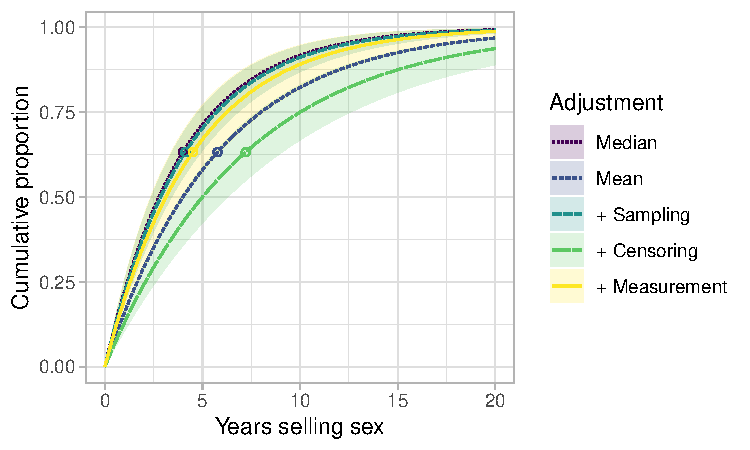
\includegraphics[scale=.75]{yss.adj}
  \caption{Estimated cumulative exponential distribution for years selling sex
    following each stage of adjustment}
  \label{fig:yss.adj}
  \floatfoot{Guide:
    \g{lines}{distributon estimate},
    \g{shaded ribbon}{\ci},
    \g{circles}{distribution mean}.
    Data from \cite{Baral2014}.}
\end{figure}
%---------------------------------------------------------------------------------------------------
\subsection{Rates of Partnership Change}\label{res.partners}
Figure~\ref{fig:partners.fsw} illustrates biased \vs unbiased estimates of
rates of partnership change ($Q$) and numbers of current partners ($K$),
% per equations \eqref{eq:bQK} \vs \eqref{eq:uQK},
based on the RDS-adjusted numbers of reported partners ($x$) in 30 days ($\omega$);
Table~\ref{tab:partners.fsw} provides the corresponding means (\ci).
The biased estimates of $Q$ and $K$ appear equal because $Q$ is defined as per-month.
We see that biases are strongest for
$Q$ with long partnerships (\eg non-paying partners) and
$K$ with short partnership (\eg new clients).
However, biases are also substantial for
both $Q$ and $K$ with ``medium-length'' partnerships (\eg regular clients).
\begin{figure}
  \centering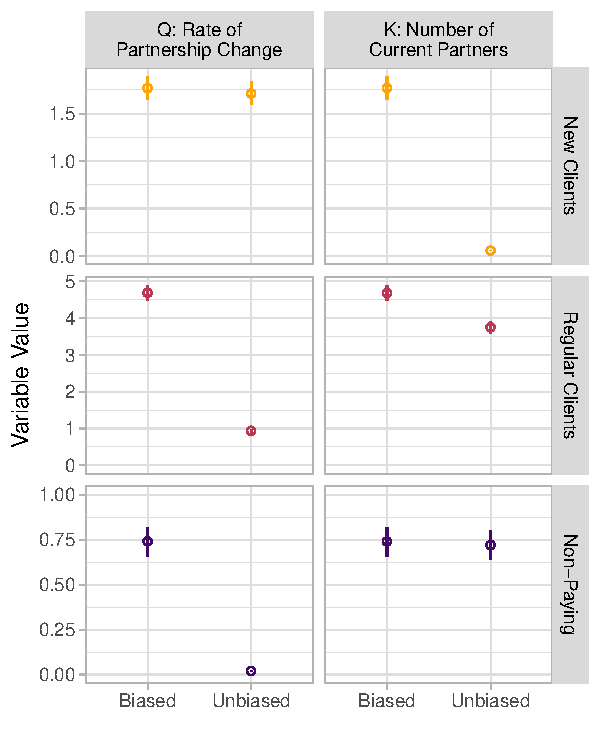
\includegraphics[scale=.8]{partners.fsw}
  \caption{Biased \vs unbiased estimates of
    rates of partnership change and numbers of current partners
    for three partnership types reported by female sex workers}
  \label{fig:partners.fsw}
  \floatfoot{Guide:
    \g{circles}{mean estimates},
    \g{bars}{\ci from 10,000 simulated surveys with $N = 328$}.
    Rates are per-month.
    Data from \cite{Baral2014}.}
\end{figure}
\par
Figure~\ref{fig:partners.sens} illustrates generalized trends in these biases,
including \ci for unbiased estimates given different simulated survey sizes $N = 10, 100, 1000$.
\begin{figure}
  \centering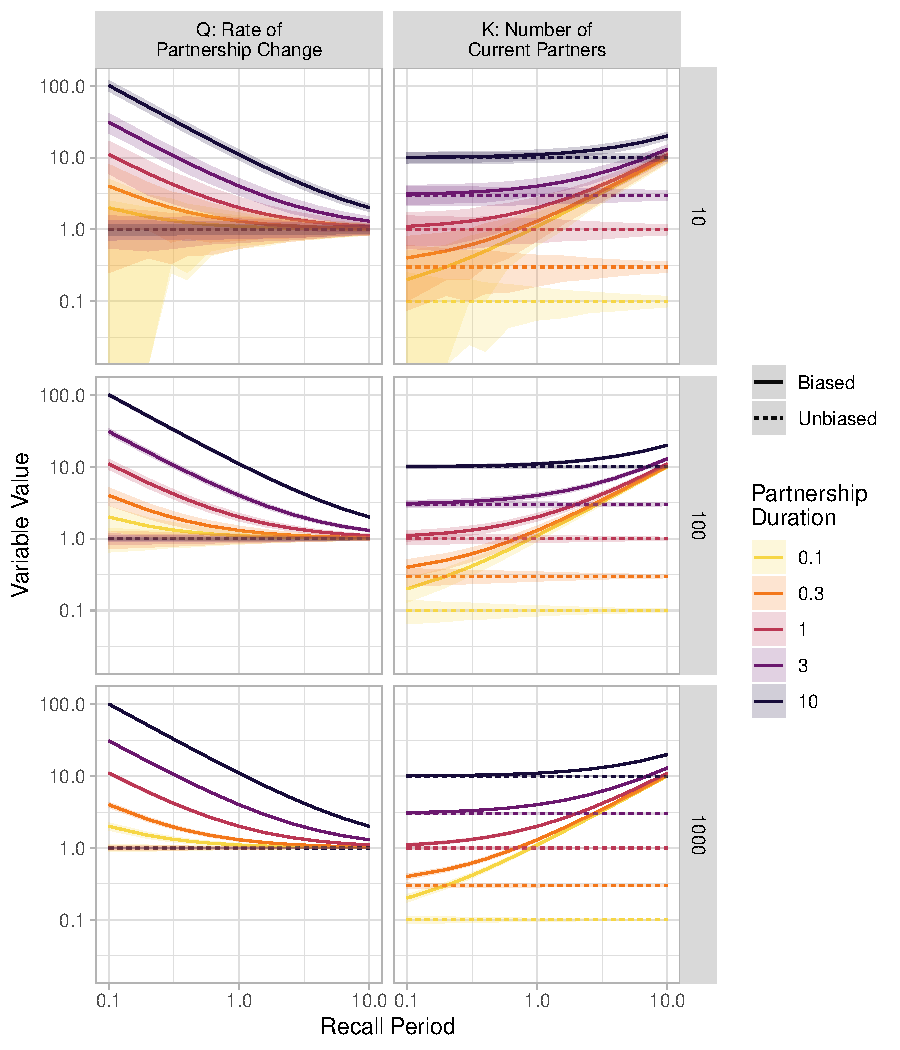
\includegraphics[scale=.8]{partners.sens}
  \caption{Biased \vs unbiased estimates of
    rates of partnership change and numbers of current partners
    for different recall periods and partnership durations}
  \label{fig:partners.sens}
  \floatfoot{Guide:
    \g{shaded ribbon}{\ci from 10,000 simulated surveys with $N = 10, 100, 1000$}.
    Units are arbitrary.}
\end{figure}
